%=========================================
% 	   Projektevaluation				 =
%=========================================
\chapter{Evaluation}
\section{Objektive Analyse der Priorisierung}
Um die Effektivität der Priorisierung zu evaluieren, soll die Anwendung der Software hier an einem Beispiel veranschaulicht werden. Nachdem sich der Benutzer registriert und angemeldet hat, können über die Seite \textit{Keywords} einige Schlüsselwörter hinzugefügt werden.
%
\medskip
\begin{figure}[!h]
    \centering
    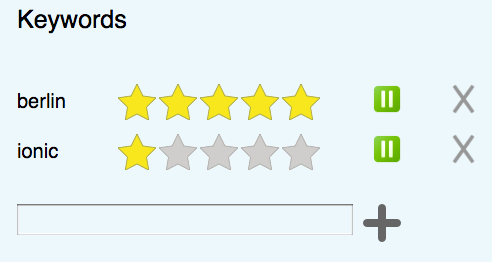
\includegraphics[width=0.65\textwidth]{Graphics/keywords}
    \caption{Konfiguration der \textit{Keywords}}
   \label{fig:keywords}
\end{figure}
%
Wie in Abbildung \ref{fig:keywords} zu sehen ist, entscheidet sich der Benutzer für die beiden Begriffe \glqq berlin\grqq{} und \glqq ionic\grqq{} und vergibt eine individuelle Priorität von fünf Sternen für \glqq berlin\grqq{} bzw. einem Stern für \glqq ionic\grqq{}. Tweets, welche dem ersten Begriff entsprechen sollten demanch eine höhere Gesamtpriorität erhalten. \\\\
Nachdem einige Tage vergangen sind, können nun die gefundenen Tweets analysiert werden. Es fällt auf, dass fast ausschließlich Tweets mit dem Keyword \glqq berlin\grqq{} angezeigt werden. Auch der in Abbildung \ref{fig:tweet_berlin} dargestellte Tweet folgt dieser Tendenz. Dies soll nun im Folgenden analysiert werden. 
%
\medskip
\begin{figure}[!h]
    \centering
    
\includegraphics[width=0.65\textwidth]{Graphics/tweet_berlin}
    \caption[Tweet: Schlüsselwort \glqq berlin\grqq{}]{Dieser Tweet wird als erster angezeigt, hat demanch die höchste Priorität}
   \label{fig:tweet_berlin}
\end{figure}
%
\newpage
Durch eine entsprechende Datenbankabfrage lässt sich herausfinden, dass der obige Tweet eine Basispriorität von 2,44 besitzt. Durch Hinzunahme der individuellen Einstufung (fünf Sterne) lässt sich diese auf 7,32 steigern. Zum Vergleich: Der am höchsten eingestufte Tweet mit dem Begriff \glqq ionic\grqq{} (vgl. Abbildung \ref{fig:tweet_ionic}) liegt mit einer Priorität von 1,42 deutlich darunter. Dieser Wert entspricht im Übrigen auch der Basispriorität, da die individuelle Einstufung durch den Faktor \glqq 1\grqq{} keine sichtbare Änderung hervorruft.
%
\medskip
\begin{figure}[!h]
    \centering
    
\includegraphics[width=0.65\textwidth]{Graphics/tweet_ionic}
    \caption[Tweet: Schlüsselwort \glqq ionic\grqq{}]{Der Tweet von \glqq ionic\grqq{} wird vergleichsweise gering bewertet}
   \label{fig:tweet_ionic}
\end{figure}
%
Auffällig ist hier insbesondere der Unterschied bei den Basisprioritäten. Trotz einer deutlich höheren \textit{Follower}-Anzahl des Autors, liegt der \glqq ionic\grqq{} Tweet hinter dem \glqq berlin\grqq{} Tweet. Dies ist auf die vergleichsweise geringe Gewichtung der \textit{Follower} zurückzuführen und explizit so gewünscht, da die Tweets eher an der Anzahl von \textit{Likes} und \textit{Retweets} gemessen werden sollen. In dem konkreten Beispiel ist die Anzahl der \textit{Retweets} (zum Zeitpunkt der Abfrage) in etwa gleich, die Anzahl der \textit{Likes} des \glqq berlin\grqq{} Tweets übertrifft seinem \glqq Konkurrenten\grqq{} jedoch um das Doppelte. \\\\
Vertauscht man die individuelle Einstufung (\glqq berlin\grqq{} : ein Stern, \glqq ionic\grqq{} : fünf Sterne), so erhöht sich die Priorität des \glqq ionic\grqq{} Tweets auf 7,1. Er liegt nun vorne.

\section{Subjektive Einschätzung der gefundenen Tweets}

Ziel des Projektes ist die automatische Selektion von Tweets unter Berücksichtigung persönlicher Interessen. Zur Evaluation dessen wird eine Woche lang nach verschiedenen Schlüsselwörtern gesucht. Dabei sind unter anderem die Begriffe \textit{Apple}, \textit{BVB} und \textit{Fender}. Bei dem Begriff \textit{Fender}, welcher eigentlich Tweets über den gleichnamigen Instrumentenbauer finden sollte, ist aufgefallen, dass größtenteils Tweets gefunden wurden, bei denen eigentliche Keyword lediglich als Infix auftritt.
%
\medskip
\begin{figure}[!h]
    \centering
    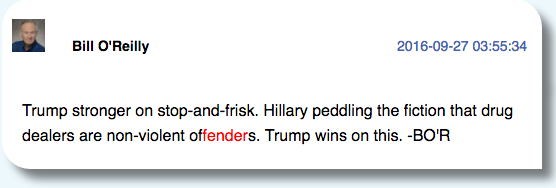
\includegraphics[width=0.65\textwidth]{Graphics/tweet_infix}
    \caption[Tweet: Schlüsselwort als Infix]{Das Keyword \textit{Fender} tritt hier nur als Teilwort auf}
   \label{fig:tweet_infix}
\end{figure}
%
Dieses Problem kann jedoch mithilfe der Suchfunktion umgangen werden. Durch die erneute Filterung tauchen nun nur noch die Tweets auf, jene das entsprechende Keyword als eigeständiges Wort enthalten. Im konkreten Beispiel tauchen nun, neben den Tweets des Herstellers selbst, vermehrt Tweets mit Bildern oder Tweets zu aktuelle Ereignissen in der Musikindustrie auf, die aber allesamt einen gewissen Informationsgehalt haben.
\\\\
Eine weitere Funktion des Programms ist das Versenden von Benachrichtigungen bei besonders interessanten Tweets. Hierzu wurde ebenfalls eine Testreihe gestartet. Das Ergebnis wird am Beispiel des Keywords \textit{BVB} verdeutlicht. In erster Linie will der Benutzer dabei über die neusten Tweets rund um den Fußballverein \textit{Borussia Dortmund} informiert werden. 
%
\medskip
\begin{figure}[!h]
    \centering
    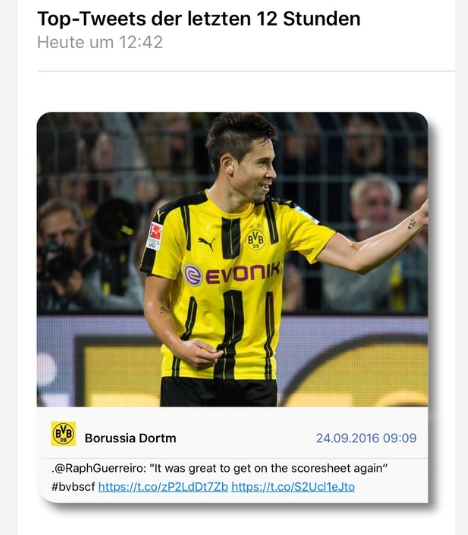
\includegraphics[width=0.65\textwidth]{Graphics/bvb_notification}
    \caption[E-Mail Benachrichtigung am Beispiel \textit{BVB}]{Nach dem Spiel wurde der Nutzer über interessante Tweets des Vereins benachrichtigt}
   \label{fig:bvb_notifications}
\end{figure}
%
Wie in Abbildung \ref{fig:bvb_notifications} zu sehen ist, wird der Benutzer kurzfristig über interessante Tweets benachrichtigt. Diese könne insgesamt als aktuell und informativ bewertet werden. Inhaltlich geht es meistens um den Fußballverein, selten ist auch ein Tweet dabei, bei dem das Keyword \textit{BVB} etwa in URLs auftaucht. Die Zeitspanne für das Senden von Benachrichtigungen (zwölf Stunden) kann aus subjektiver Sicht als zu gering betrachtet werden, da nicht immer interessante Ereignisse stattfinden und dadurch eine gewisse Menge an irrelevanten Tweets zustande kommt.









